\chapter{Adding Memory to the Agents}
\section{Overview}
In the previous chapters, we have assumed that the agents interact in fully observable problems, following an MDP. This means that the observation that the agent receives from the environment is sufficient to fully understand its state. Thus:

\begin{equation}
    s_{t} = o_{t}
\end{equation}

However, this is not always true. In robotics problems, robots observe its environment through sensors, and, commonly, the data obtained from them gives partial information about the robot's state. So, a significant set of real-world problems is better described by Partially Observable Markov Decision Processes (POMDPs).

There are different reason of why a problem could be partially observed. One of them is when a state is described by time-dependent phenomena, and the observations only get partial information about them. For instance, an agent could need to estimate the velocity of a flying drone by getting instant RGB snapshots of its movements. Unless observations from different time steps are combined, the agent is not going to be able to make this estimation. Other examples of time-dependent phenomena that do not have to do with the dynamics of the environment are temporary occlusions or corrupted communication systems between the sensors and the agent. From now on, we are going to use the acronym POMDP to refer to the just mentioned set of problems.

All of these scenarios are not covered by the variations of D-COACH proposed so far. In this chapter, we aim to add memory to the policies trained with D-COACH, in order to have a system capable of solving sequential decision-making problems with partially observed time-dependent states. The idea is to validate this approach through simulations, establishing a baseline for further research in memory-based deep interactive learning.
\newpage

\section{Methodology}
There are two well-known approaches for adding memory to agents in sequential decision-making problems when using DNNs as function approximators:

\begin{enumerate}
    \item \textbf{Observation stacking \cite{atari}}: This approach consists in stacking a fixed number of past observations to the current one and using this stack as the input of the policy. 
    \item \textbf{Recurrent models \cite{hausknecht2015deep}:} This approach uses policies that incorporate RNN layers into its neural network architecture. Given that these models have an internal state, they can store information from the past (i.e. they have memory) and use it in future inferences. 
\end{enumerate}

One of the main issues of observation stacking is that the memory of these models is determined by the number of stacked observations. Problems that need to remember events in medium or large sequences would require larger stacks. In high-dimensional state problems, the size of the input can increase considerably as the number of stacked observations increments, generating high overheads. In contrast, RNN-based models have the ability to remember information for an arbitrarily long amount of time \cite{lample2017playing}. Also, they have no input-related overheads because when these models are evaluated they use as input one observation at a time. In RNNs, the memory-related overhead is determined by the size of their hidden states and the length of the sequences used when updating the weights of the models, so the latter is only effective when training.

From an engineering point of view, using RNNs in products for real-world applications with long or medium time dependencies could lower their costs in comparison to using observation stacking. The input overhead of approaches based on stacked observations would be too high in these scenarios; thus, more powerful (expensive) computers would be needed. 

Given the more practical usage of recurrent models and their capability of representing arbitrarily long sequences, in this chapter we use RNN-based policies (with LSTM layers) to test the viability of D-COACH for solving problems in POMDP settings. 

\subsection{Learning to Remember}
Even though RNNs are networks with the capability of storing information from past observations, they have to learn to do this. Commonly, in DRL approaches this is implicitly learned when backpropagating the error that aims to maximize the expected return. This gives the intuition that when using D-COACH, backpropagating the correction error through the recurrent layers should be enough for learning well-performing policies. Nevertheless, preliminary tests showed that shaping recurrent models with corrective feedback made the agents to rapidly overfit to the first set of corrections, loosing the capability of learning interesting behaviors and, as a consequence, failing to solve the tasks. 

To overcome this problem, we propose to have DNNs separated into two parts: (1) transition model and (2) policy. The transition model is in charge of learning the dynamics of the environment in a supervised manner using samples collected by the agent while the policy part is shaped using corrective feedback. 

In MDPs, a transition model is capable of predicting the next state of the environment as a function of the current state and the taken action $M(s_{t},a_{t}) = s_{t+1}$ (as in Equation \ref{eq:model}). In contrast, in POMDPs the agent does not have direct access to its state, so, instead, the transition model can be trained to predict the next observation $o_{t+1}$. To achieve this, the neural network architecture must include recurrent layers (LSTMs in this case). LSTMs can represent in their hidden state $h_{t}$ information from past observations, which is crucial to predict the next observation when the environment is partially observed. Thus, the objective of the first part of the DNN is to learn $M(o_{t},a_{t}, h_{t-1}) = \widetilde o_{t+1}$, which, as a consequence, learns to embed past observations in $h_{t}$.

The second part of the DNN, the policy, takes as input the concatenation of the hidden state of the transition model computed in the last time step $h_{t-1}$ with the current observation of the environment $o_{t}$ and uses this information as if it were the state. D-COACH is used to update the weights of this part as it is done in fully-observable low-dimensional state problems with D-COACH OFF. In this chapter, we are assuming that a representation of past observations combined with the current observation is a good approximation of $s_{t}$:

\begin{equation}
s_{t}\approx (h_{t-1}, o_{t})    
\end{equation}

We call this approach Memoryful ONline state representation learning D-COACH (D-COACH MON). A summary of this approach is presented in Figure \ref{fig:mb_dcoach}.

\begin{figure}[h]
    \centering
    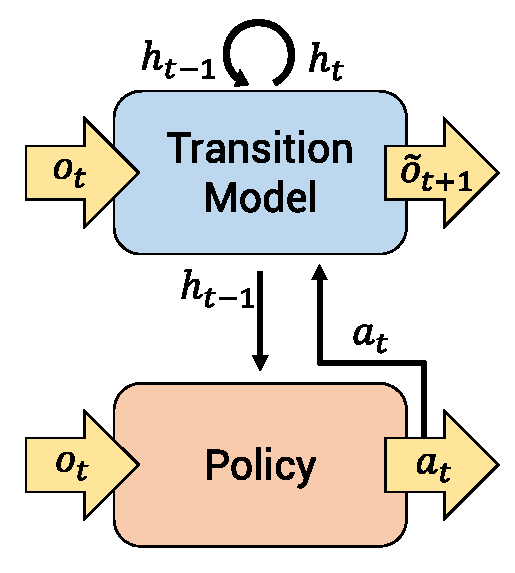
\includegraphics[width=0.4\linewidth]{imagenes/cap4/model_based_dcoach.pdf}
    \caption{D-COACH MON general structure.}
    \label{fig:mb_dcoach}
\end{figure}

\newpage

\subsection{Low-dimensional State with Memory}
\label{sec:ld_memory}
As it has been done previously in this work, we first study the low-dimensional state case. The objective is to learn the dynamics of the environment online i.e. as the policy is shaped interactively. 

If we look back to the approach taken in Chapter 3, the idea was similar. In that case the objective was to learn a low-dimensional representation of a high-dimensional input online. The strategy was to share the encoder layers of an autoencoder between the policy and the autoencoder, and to update them using both the cost of the policy and the one of the autoencoder. In this case, the hidden state of the LSTM could be interpreted as a representation of past observations. So, this recurrent layers could be shared between the policy and the model, updating them using both costs. A simplified version of this approach is shown in Figure \ref{fig:ld_model_rip}.

\begin{figure}[h]
    \centering
    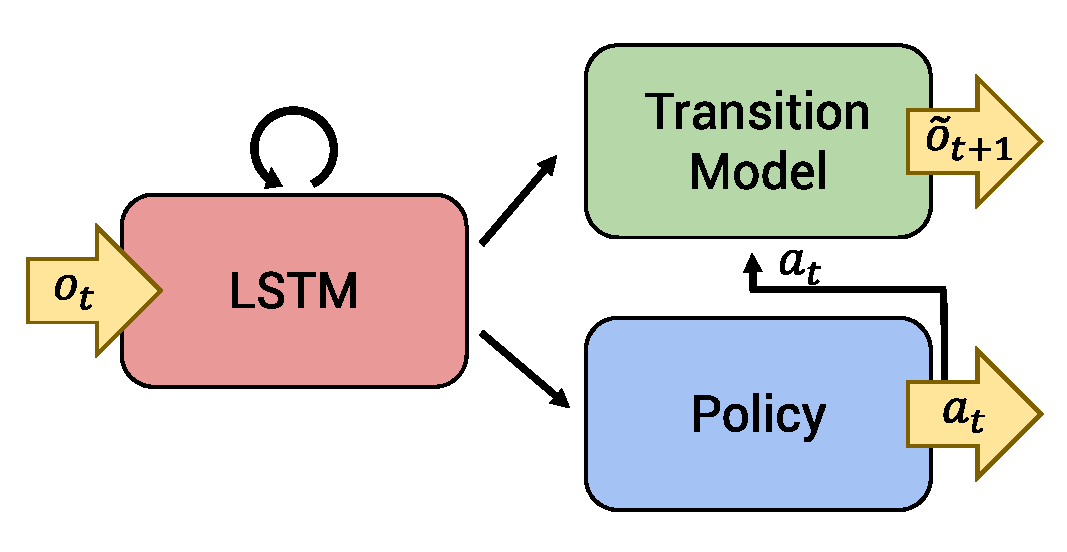
\includegraphics[width=0.6\linewidth]{imagenes/cap4/ld_model_rip.pdf}
    \caption{Low-dimensional observations general neural network architecture for POMDPs (option 1).}
    \label{fig:ld_model_rip}
\end{figure}

The shortcoming presented in the approach shown in Figure \ref{fig:ld_model_rip} is that in this case the same problem that we found in the preliminary tests appears. The error of the policy does not work well when updating the weights of recurrent layers using the D-COACH strategy, even when using the auxiliary cost of the model. 

Alternatively, the approach that was finally taken was to update the model and the policy separately and simultaneously. If we go back to Figure \ref{fig:mb_dcoach}, this would mean that the \textbf{Transition Model} box is updated with transitions collected by the agent, and, separately, the \textbf{Policy} box is updated with corrective feedback. The proposed transition model architecture (\textbf{Transition Model} box in Figure \ref{fig:mb_dcoach}) consists of LSTM and FNN layers, as shown in Figure \ref{fig:ld_model_win}. The policy architecture (\textbf{Policy} box) is simply a composition of FNN layers, as it is done in the other variations of D-COACH.

\newpage

\begin{figure}[H]
    \centering
    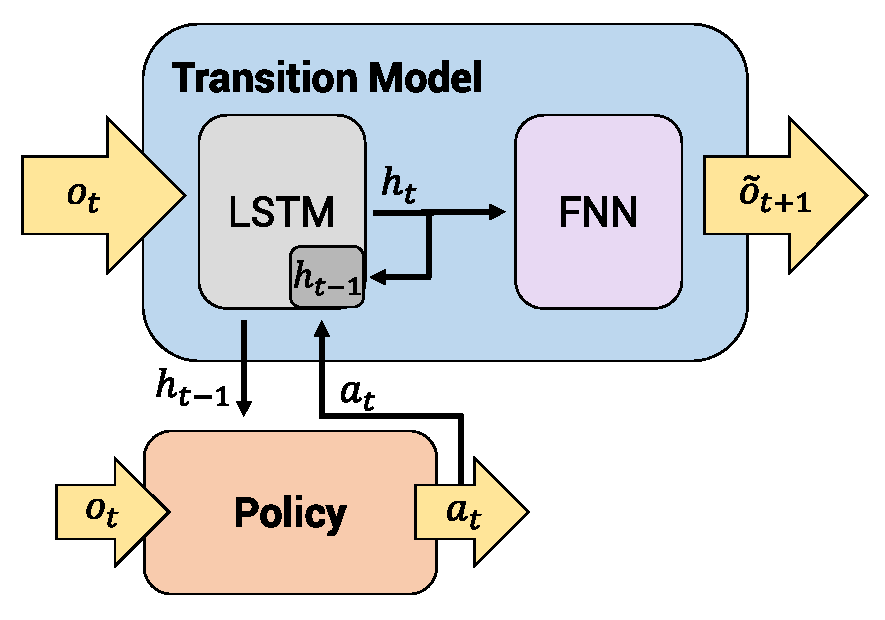
\includegraphics[width=0.5\linewidth]{imagenes/cap4/ld_model.pdf}
    \caption{Low-dimensional observations general neural network architecture for POMDPs (option 2).}
    \label{fig:ld_model_win}
\end{figure}

Figure \ref{fig:ld_model_win} presents the general structure of the neural network architecture that is proposed for problems with low-dimensional observations. A detailed version of the network architecture is provided in Figure \ref{fig:detailed_ld}.

\begin{figure}[h]
    \centering
    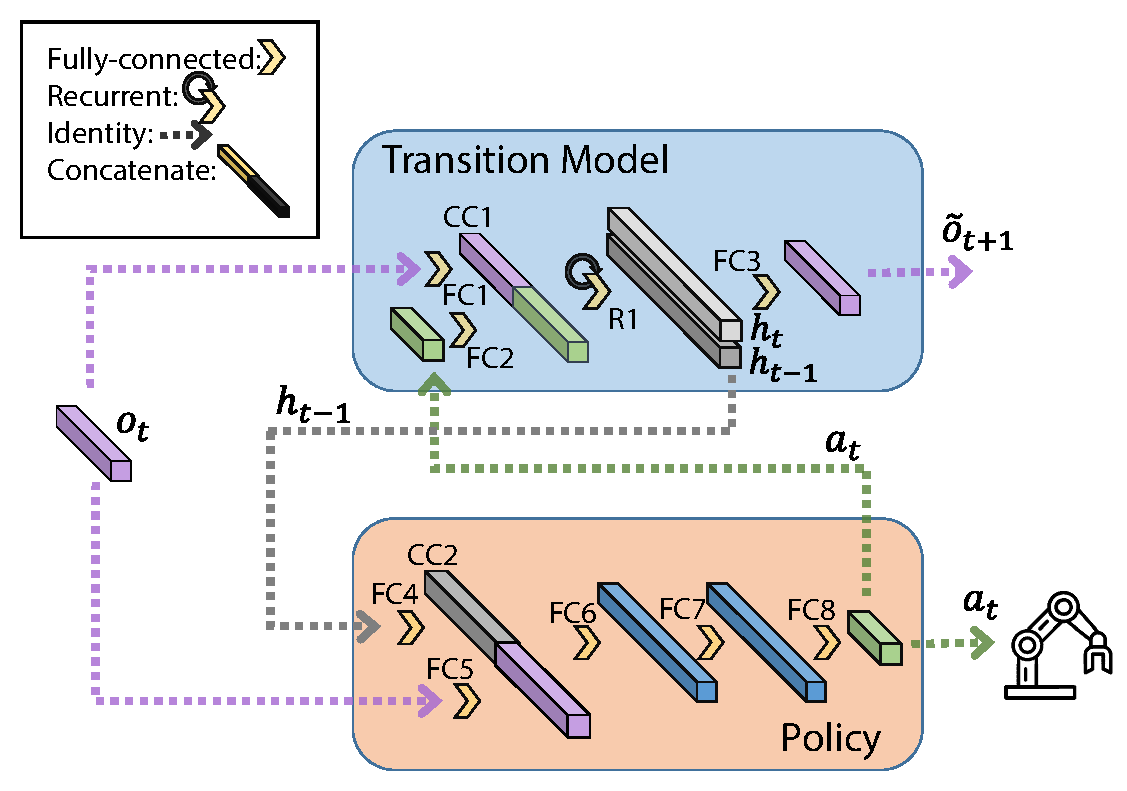
\includegraphics[width=0.8\linewidth]{imagenes/cap4/ld_model_det.pdf}
    \caption{D-COACH MON low-dimensional observations neural network architecture.}
    \label{fig:detailed_ld}
\end{figure}

As mentioned before, the transition model and the policy are trained as two separate networks. These networks depend on each other. The policy uses as part of its input $h_{t-1}$, which is a vector that the transition model outputs. Similarly, the transition model uses the last taken action as part of its input, which is a vector generated by the policy. When an update of the architecture is done, the transition model is first updated, and, consecutively, the policy is updated. A summary of this process is presented in Figure \ref{fig:ld_mon_train}.

\begin{figure}[h]
\centering
\subfloat[][Transition model update step.]{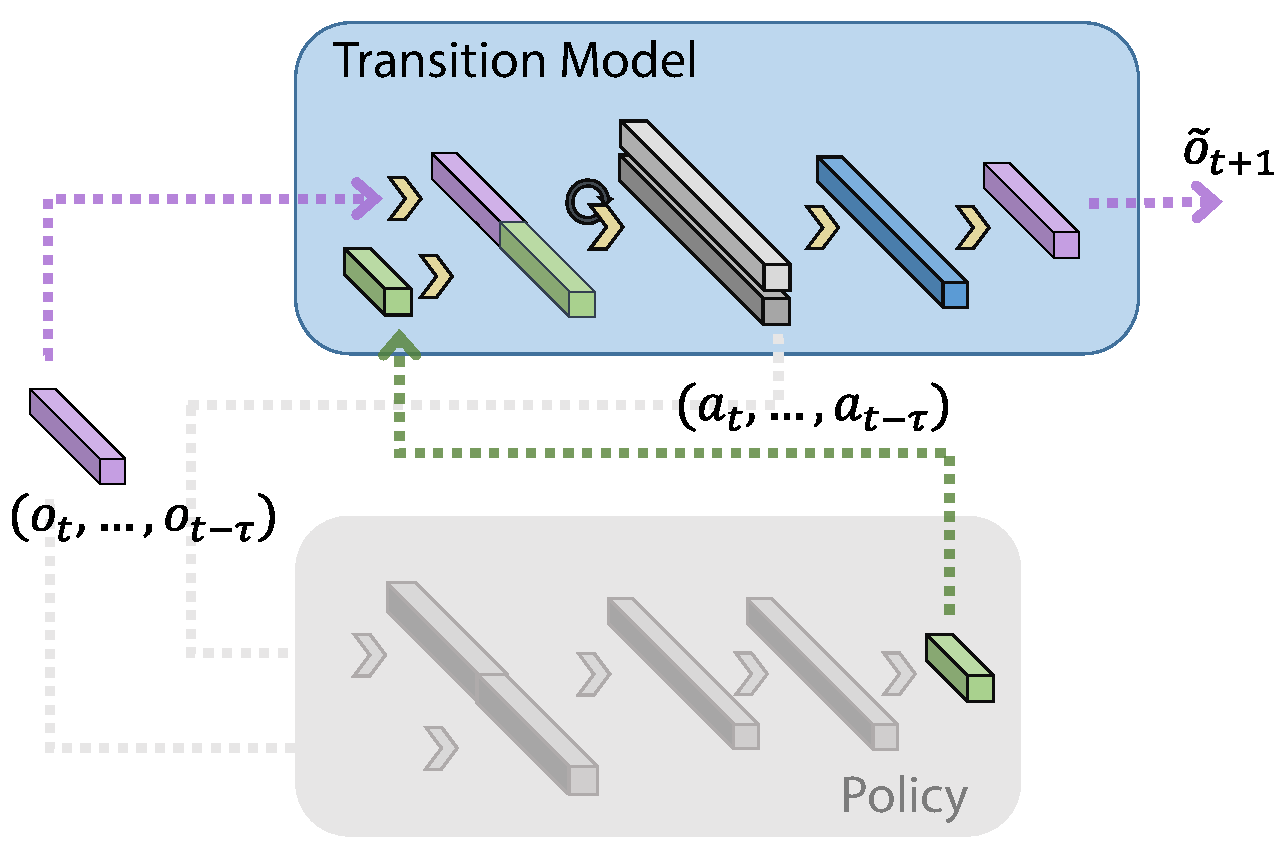
\includegraphics[width=0.49\linewidth]{imagenes/cap4/ld_mon1.pdf}}
\subfloat[][Policy update step.]{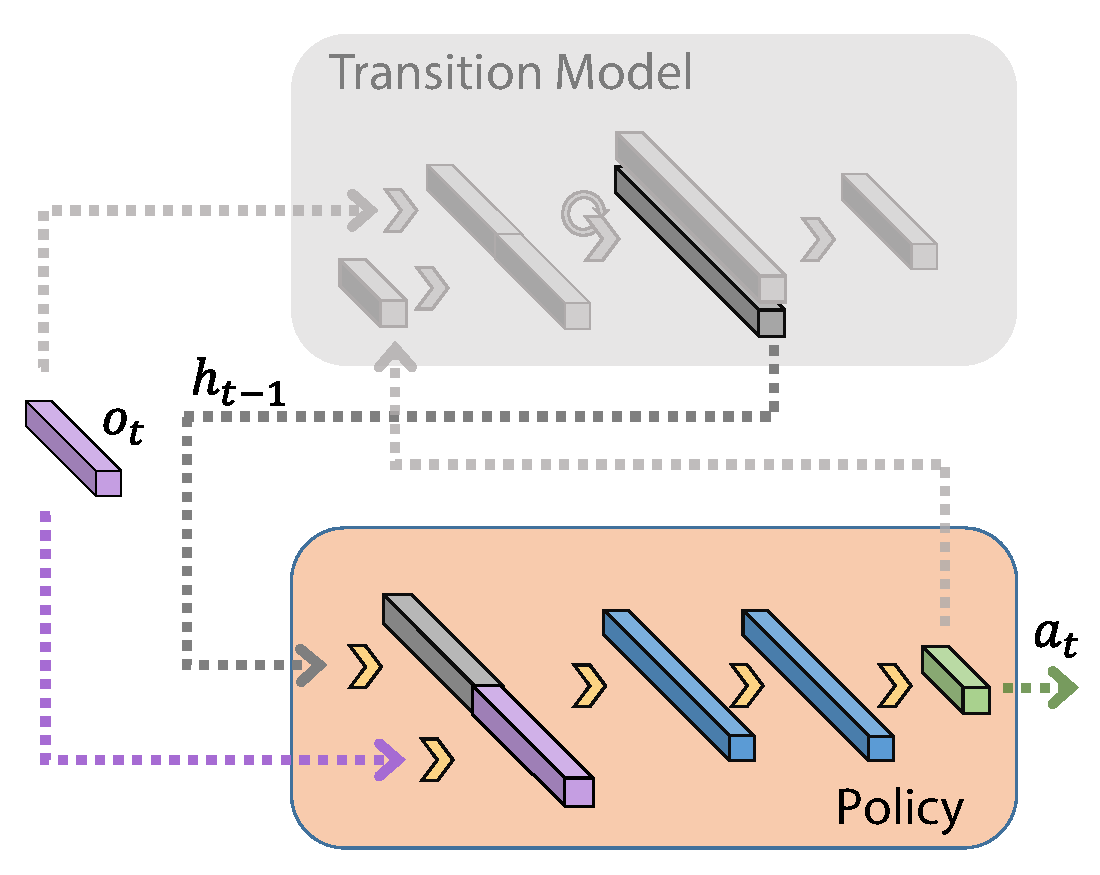
\includegraphics[width=0.45\linewidth]{imagenes/cap4/ld_mon2.pdf}}
\caption[Update step of D-COACH MON neural network for low-dimensional observations.]{Update step of D-COACH MON neural network for low-dimensional observations. First (a), the transition model is updated in a supervised manner using as input a batch with sequences of observations and actions where the labels correspond to $o_{t+1}$. Consecutively (b), the policy is updated using human corrective feedback using as input $o_{t}$ and $h_{t-1}$.} 
\label{fig:ld_mon_train} 
\end{figure}

\subsection{High-dimensional State with Memory}
In the high-dimensional case, agents need to learn two representations: (1) spatial and (2) temporal. Spatial representation are understood as a low-dimensional representation of high-dimensional data, which is what it has been covered in the former chapters using autoencoders. In contrast, temporal representations refer to encapsulating previous observations in a memory, which is what it has been done in Section \ref{sec:ld_memory} using LSTMs. 

In preliminary tests, we found that the most effective way of doing this under the setting of D-COACH is to treat the autoencoder and the recurrent layers as one architecture to represents the transition function model. A model with the capability of learning from high-dimensional states, as it can be seen in Figure \ref{fig:rnn_hd}. 

\begin{figure}[h]
    \centering
    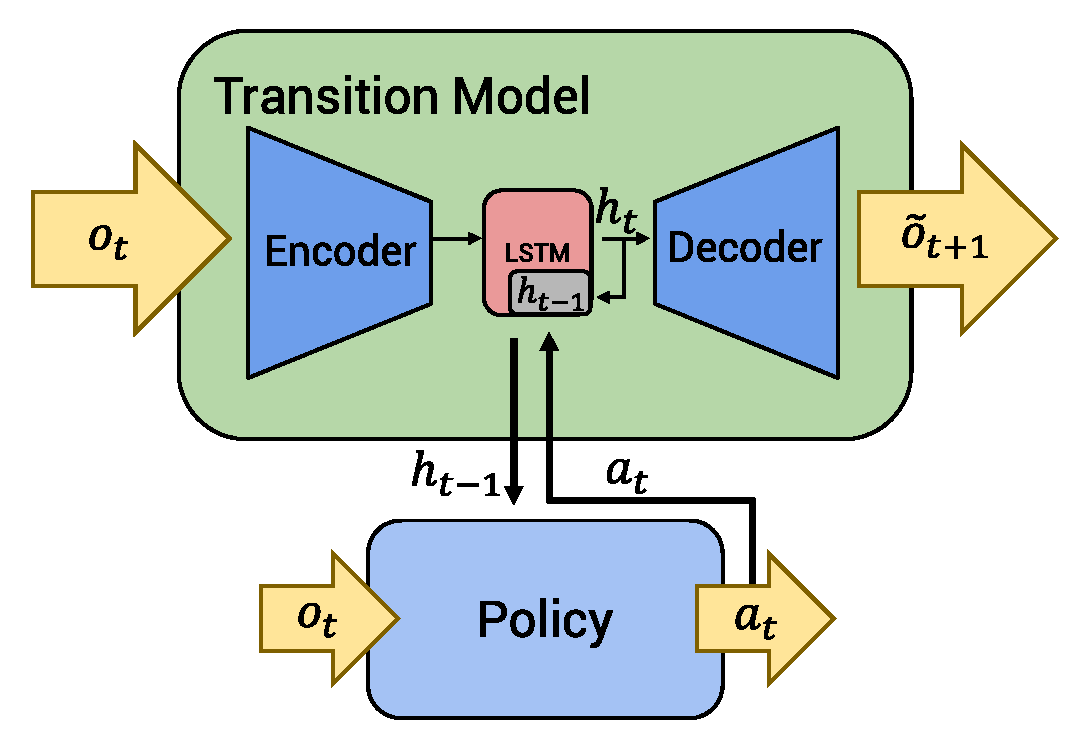
\includegraphics[width=0.5\linewidth]{imagenes/cap4/hd_model.pdf}
    \caption{High-dimensional observations general neural network architecture for POMDPs.}
    \label{fig:rnn_hd}
\end{figure}

Instead of using separate costs for the model and the autoencoder, the autoencoding cost for reconstructing $o_{t+1}$ is used. So, Equation \ref{eq:ae} instead of being $L(x_{t},\widetilde x_{t})$ it would be  $L(x_{t},\widetilde x_{t+1})$. By doing this, the hidden state of the LSTM represents both the high-dimensional input and past observations, given that the autoencoder tries to reconstruct and predict $o_{t+1}$. As it was done for the low-dimensional observation case, Figure \ref{fig:detailed_hd} introduces the detailed neural network architecture for the high-dimensional observation case.

\begin{figure}[h]
    \centering
    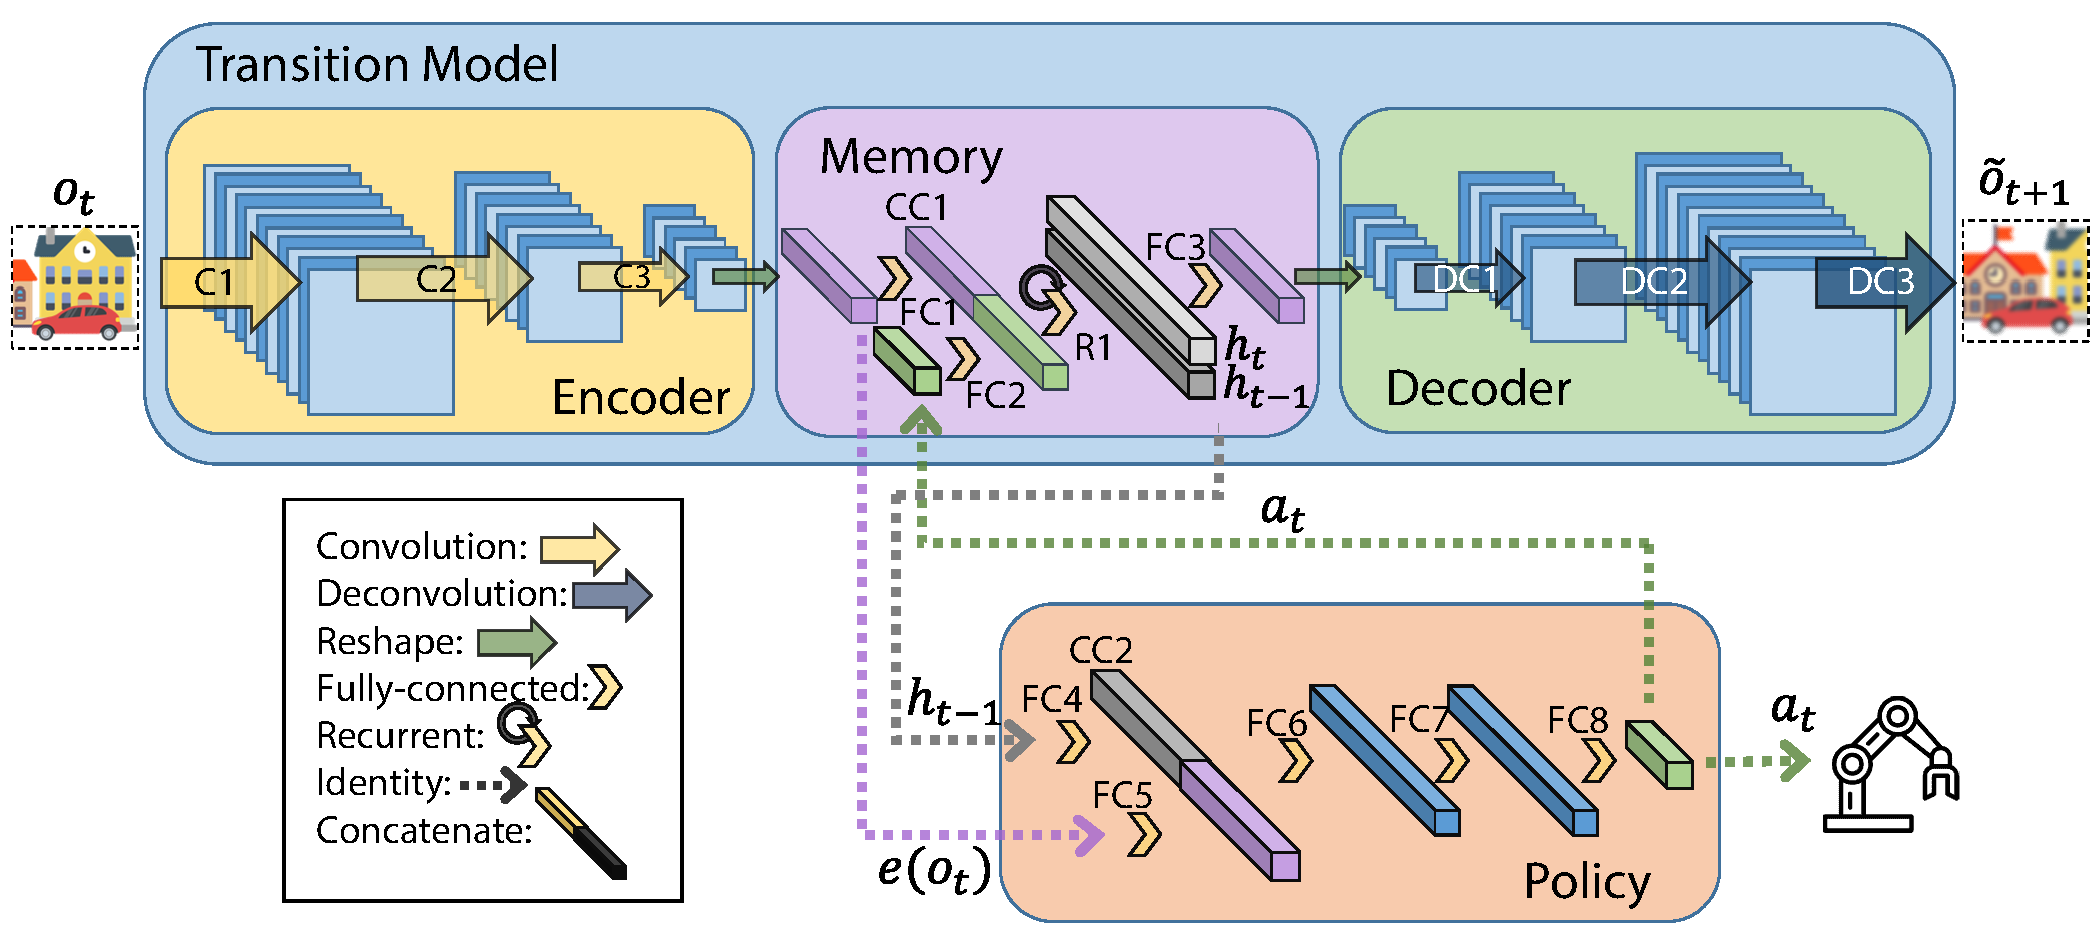
\includegraphics[width=\linewidth]{imagenes/cap4/hd_model_det.pdf}
    \caption{D-COACH MON high-dimensional observations neural network architecture.}
    \label{fig:detailed_hd}
\end{figure}

In the same way as in the low-dimensional observation case, the transition model and the policy are trained separately and simultaneously. The only difference is that in this case, when the policy is updated it uses the encoding layers to generate an encoded low-dimensional representation of the observation $e(o_{t})$ that the policy uses as input, but only the policy layers are updated. This is also different from what is done in D-COACH OFF, where the encoding layers are also updated when training the policy. Figures \ref{fig:hd_mon_train1} and \ref{fig:hd_mon_train2} summarize a D-COACH MON update step for high-dimensional observations.

\begin{figure}[h]
    \centering
    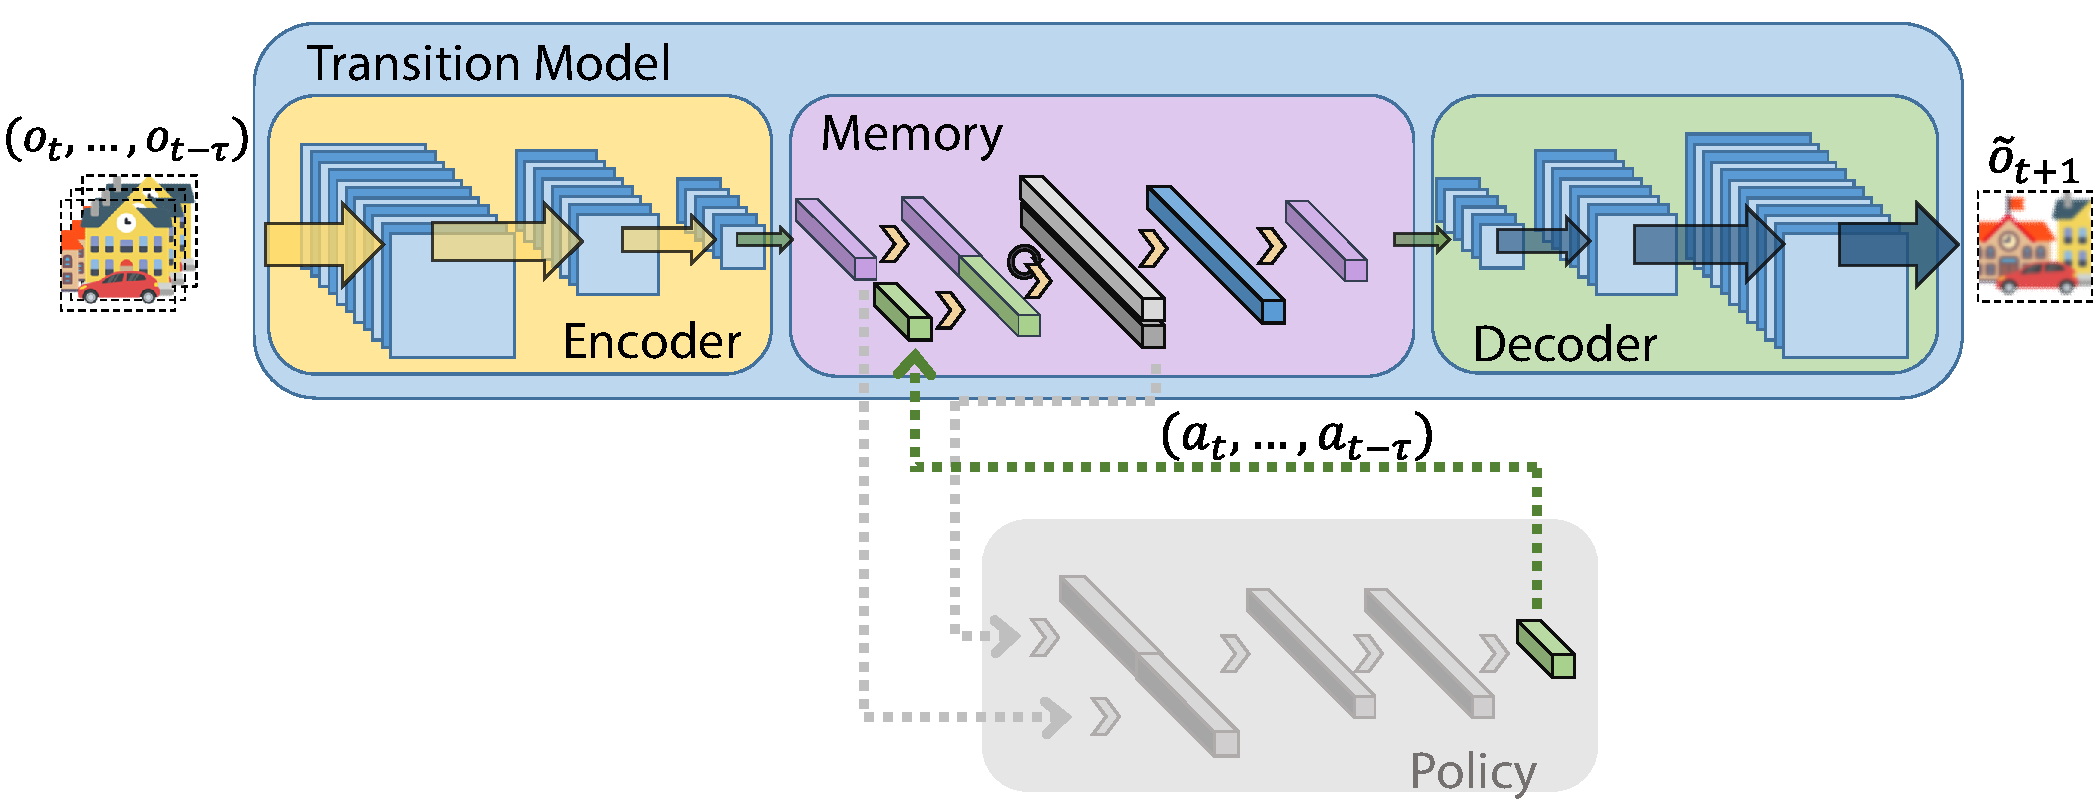
\includegraphics[width=0.93\linewidth]{imagenes/cap4/hd_mon1.pdf}
    \caption{Transition model update step.}
    \label{fig:hd_mon_train1}
\end{figure}

\begin{figure}[h]
    \centering
    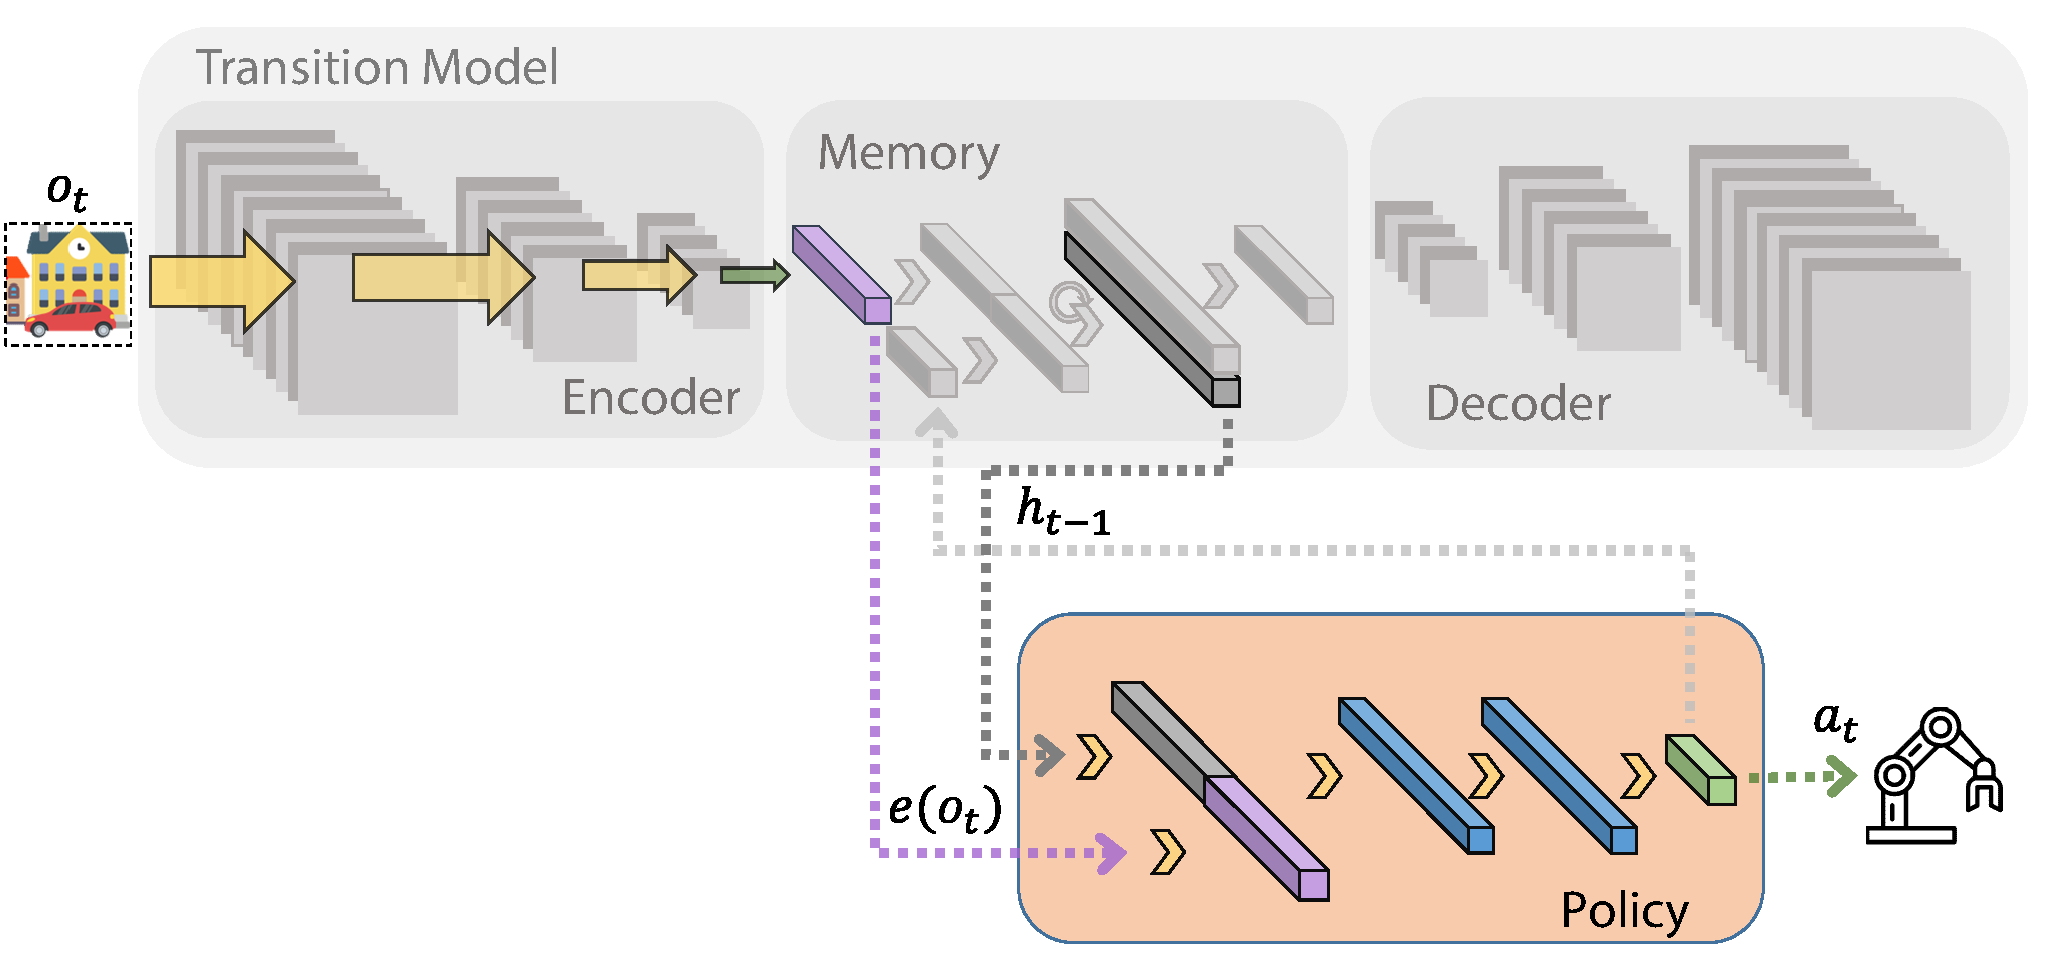
\includegraphics[width=0.93\linewidth]{imagenes/cap4/hd_mon2.pdf}
    \caption{Policy update step.}
    \label{fig:hd_mon_train2}
\end{figure}


\subsection{The Algorithm}

In Algorithm \ref{algorithm:DeepCOACH-M}, the pseudocode of D-COACH MON is presented. The hidden state of the LSTM is denoted as  $h^{\mathrm{LSTM}}$ and the human corrective feedback as $h$.

In every time step, the agent executes an action based on its last observation and in the current hidden state of the LSTM (line 5). This hidden state is updated using its previous value and the most recent observation and action (line 7). In this occasion, a buffer in charge of storing the samples of the transition function model ($\mathcal{D}$) is incorporated. In both buffers, $\mathcal{B}$ and $\mathcal{D}$, sequences with length $\tau$ are stored (lines 8 and 18), which is necessary for training the LSTM. This is done following the \emph{bootstrapped random updates} \cite{hausknecht2015deep} strategy. As in the former versions of D-COACH, $\mathcal{B}$ is used for updating the policy (lines 16 and 22) by replaying past corrections. In contrast, $\mathcal{D}$ replays past transitions of the environment in order to update the transition function model (lines 17 and 24). The transition model is updated every time feedback is given (lines 15 and 17), in the same way as it is done with the policy in all of the variations of D-COACH, including this one (lines 14 and 16). 

\begin{algorithm}[H]
\caption{D-COACH MON: Memoryful Online State Representation Learning}\label{algorithm:DeepCOACH-M}
\begin{algorithmic}[1]
\State \textbf{Require:} error magnitude $e$, policy buffer update interval $b$, policy buffer sampling size $N$, policy buffer min. size $k$, policy buffer max. size $K$, model buffer update interval $d$, transition function model buffer sampling size $M$, transition function model buffer min. size $l$, transition function model buffer max. size $L$, training sequence length $\tau$.
\State \textbf{Init:} $\mathcal{B} = []$, $\mathcal{D} = []$
\For{t = 1,2,...}{}
\State \textbf{observe} observation $o_{t}$
\State \textbf{execute} action $a_{t}=\pi(o_{t}, h^{\mathrm{LSTM}}_{t-1})$
\State \textbf{feedback} human corrective advice $h_{t}$
\algstore{myalg}
\end{algorithmic}
\end{algorithm}

\begin{algorithm}            
\begin{algorithmic} [1]                  
\algrestore{myalg}
\State \textbf{compute} $h^{\mathrm{LSTM}}_{t}$ from $M(o_{t}, a_{t},h^{\mathrm{LSTM}}_{t-1})$
\State \textbf{append} $(o_{t-1},...,o_{t-\tau},a_{t-1},...,a_{t-\tau},o_{t})$ to $\mathcal{D}$
\If{length($\mathcal{D}$) $> L$ }
\State $\mathcal{D} = \mathcal{D}[2:L+1]$
\EndIf
\If{$h_{t}$ is not \textbf{0}}
\State $\mathit{error}_{t} = h_{t}\cdot e$
\State $y_{label(t)} = a_{t} + \mathit{error}_{t}$ 
\State \textbf{update} $\pi$ using SGD with $(o_{t}, h^{\mathrm{LSTM}}_{t-1}, y_{\mathit{label}(t)})$ 
\State \textbf{update} $M$ using SGD with $(o_{t-1},...,o_{t-\tau},a_{t-1},...,a_{t-\tau},o_{t})$
\State \textbf{update} $\pi$ using SGD with a mini-batch of sequences sampled from $\mathcal{B}$
\State \textbf{update} $M$ using SGD with a mini-batch of sequences sampled from $\mathcal{D}$
\State \textbf{append} $(o_{t},...,o_{t-\tau},a_{t-1},...,a_{t-\tau}, y_{\mathit{label}(t)})$ to $\mathcal{B}$
\If{length($\mathcal{B}$) $> K$ }
\State $\mathcal{B} = \mathcal{B}[2:K+1]$
\EndIf
\EndIf
\If{mod(t, b) is 0 and length($\mathcal{B}$) $\geq$ $k$}
\State \textbf{update} $\pi$ using SGD with a mini-batch of sequences sampled from $\mathcal{B}$
\EndIf
\If{mod(t, d) is 0 and length($\mathcal{D}$) $\geq$ $l$}
\State \textbf{update} $M$ using SGD with a mini-batch of sequences sampled from $\mathcal{D}$
\EndIf
\EndFor
\end{algorithmic}
\end{algorithm}


\section{Experiments and Results}
Simulated teachers were used in three different problems for validating D-COACH MON. The main idea behind these experiments is to compare D-COACH MON with D-COACH ON in partially observable problems.

\begin{enumerate}
    \item \textbf{Partially Observed Cart-Pole:} A partially observed low-dimensional observation scenario. This is the same environment used in Chapter 3 with a modification in the observation space of the agent. In the standard fully-observable cart-pole the state has four dimensions, which consists of the position $x$ and velocity $\dot x$ of the cart and the angle $\theta$ and angular velocity $\dot \theta$ of the pole, such that $s=[x, \dot x, \theta, \dot \theta]$. In this case, we take out the derivatives present in the state, such that $s=[x, \theta]$.
    \item \textbf{Partially Observed Cart-Pole from Pixels:} The Cart-Pole environment is modified to use as input raw pixels from an image with dimensions $32\times32\times1$ (high-dimensional state). 
    \item \textbf{Partially Observed Car Racing:} A partially observed high-dimensional state scenario. The Car Racing problem presented in Chapter 2 is modified such that the indicators in the bottom of the image are no longer available (see Figure \ref{fig:no_inds_car_racing}). 
\end{enumerate}

\begin{figure}[h]
    \centering
    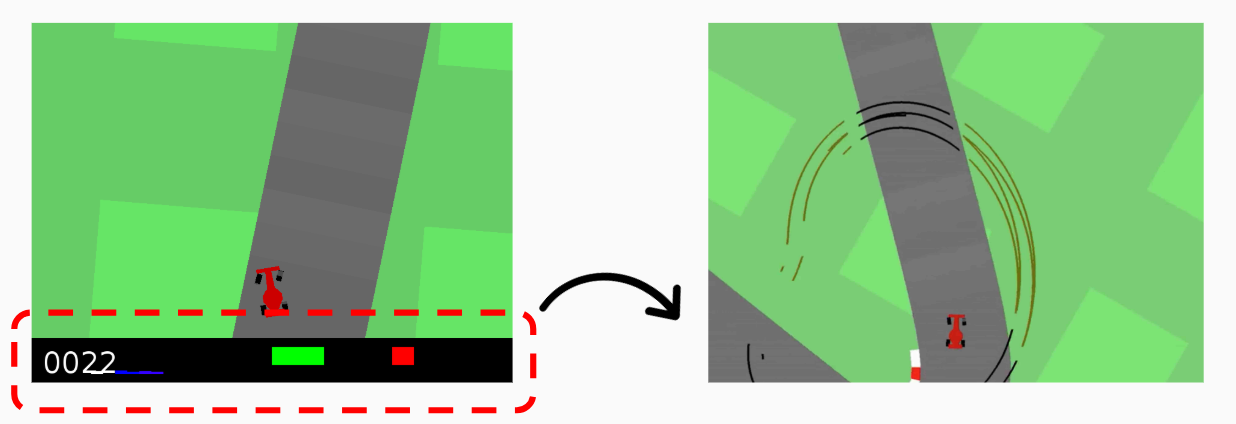
\includegraphics[width=0.7\linewidth]{imagenes/cap4/car_racing_no_inds.PNG}
    \caption[Partially observed Car Racing.]{Partially observed Car Racing: indicators at the bottom of the observation are removed.}
    \label{fig:no_inds_car_racing}
\end{figure}

All the results that present averaged data in the form of a curve have confidence intervals that represent the $60^{th}$ percentile of the data. For problems with low-dimensional observations, the neural network architecture presented in Figure \ref{fig:detailed_ld} was used, and the hyper-parameters values are shown in Table \ref{table:mon_ld_hyp}. For the high-dimensional observation case, the neural network architecture introduced in \ref{fig:detailed_ld} was, and the hyper-parameters shown in Tables \ref{table:mon_hypers1}, \ref{table:mon_hypers2} and \ref{table:mon_hypers3} were used. The rows in the tables with no values were not used i.e. replace FC with identity. In the same way as in Chapter 3, the hyper-parameters of the neural networks used in these experiments were tuned with preliminary experiments.

\begin{table}[]
\centering
\caption[Low-dimensional observation D-COACH MON neural network hyper-parameters.]{D-COACH MON low-dimensional observation neural network hyper-parameters.}
\label{table:mon_ld_hyp}
\begin{tabular}{lcc}
\textbf{Layer}                                              & \multicolumn{1}{l}{\textbf{Activation}} & \multicolumn{1}{l}{\textbf{$N^{\circ}$ neurons}}                \\ \hline \hline
FC1                                                         & ---                                     & ---                                                    \\ \hline
FC2                                                         & ---                                     & ---                                                    \\ \hline
FC3                                                         & ReLU                                    & 300                                                    \\ \hline
\begin{tabular}[c]{@{}l@{}}FC4\\ (size obs.)\end{tabular}   & tanh                                    & Part. Cart-Pole: 2                                     \\ \hline
FC5                                                         & ---                                     & ---                                                    \\ \hline
FC6                                                         & ReLU                                    & 150                                                    \\ \hline
FC7                                                         & ReLU                                    & 64                                                     \\ \hline
FC8                                                         & ReLU                                    & 64                                                     \\ \hline
\begin{tabular}[c]{@{}l@{}}FC9\\ (size action)\end{tabular} & tanh                                    & Part. Cart-Pole: 1                                     \\ \hline
R1                                                          & LSTM                                    & \begin{tabular}[c]{@{}c@{}}150\\ (size h)\end{tabular} \\ \hline
\end{tabular}
\end{table}

\begin{table}[H]
\parbox{\linewidth}{
\centering
\caption[High-dimensional observation D-COACH MON convolutional and deconvolutional layers hyper-parameters]{D-COACH MON high-dimensional observations convolutional and deconvolutional layers hyper-parameters. Autoencoder latent space size: $8\times8\times4$ (Car Racing) and $4\times4\times4$ (HD Cart-Pole).}
\label{table:mon_hypers1}
\begin{tabular}{lcccc}
\textbf{Layer} & \multicolumn{1}{l}{\textbf{Activation}} & \multicolumn{1}{l}{\textbf{Filters}} & \multicolumn{1}{l}{\textbf{Filter size}} & \multicolumn{1}{l}{\textbf{Stride}} \\ \hline \hline
C1             & ReLU                                    & 16                                   & $3\times3$                                    & 2                                   \\ \hline
C2             & ReLU                                    & 8                                    & $3\times3$                                    & 2                                   \\ \hline
C3             & ReLU                                    & 4                                    & $3\times3$                                    & 2                                   \\ \hline
DC1            & ReLU                                    & 8                                    & $3\times3$                                    & 2                                   \\ \hline
DC2            & ReLU                                    & 16                                   & $3\times3$                                    & 2                                   \\ \hline
DC3            & ReLU                                    & 1                                    & $3\times3$                                    & 2                                   \\ \hline
\vspace{0.2cm}
\end{tabular}}
\end{table}

\begin{table}
\parbox{.45\linewidth}{
\centering
\caption{High-dimensional observation D-COACH MON fully-connected and LSTM layers hyper-parameters.}
\label{table:mon_hypers2}
\begin{tabular}{lcc}
\textbf{Layer}                                              & \multicolumn{1}{l}{\textbf{Activation}} & \multicolumn{1}{l}{\textbf{$N^{\circ}$ neurons}}                                        \\ \hline
FC1                                                         & ---                                     & ---                                                                                     \\ \hline
FC2                                                         & ---                                     & \begin{tabular}[c]{@{}c@{}}Car Racing: 256\\ HD Cart-Pole: 64\end{tabular} \\ \hline \hline
FC3                                                         & ReLU                                    & 300                                                                                     \\ \hline
FC4                                                         & ReLU                                    & \begin{tabular}[c]{@{}c@{}}Car Racing: 256\\ HD Cart-Pole: 64\end{tabular} \\ \hline
FC5                                                         & ReLU                                    & 150                                                                                     \\ \hline
FC6                                                         & ReLU                                    & 150                                                                                     \\ \hline
FC7                                                         & ReLU                                    & 64                                                                                      \\ \hline
FC8                                                         & ReLU                                    & 64                                                                                      \\ \hline
\begin{tabular}[c]{@{}l@{}}FC9\\ (action size)\end{tabular} & tanh                                    & \begin{tabular}[c]{@{}c@{}}Car Racing: 3\\ HD Cart-Pole: 1\end{tabular}     \\ \hline
R1                                                          & LSTM                                    & \begin{tabular}[c]{@{}c@{}}150\\ (size h)\end{tabular}                                  \\ \hline
\end{tabular}}
\hfill
\parbox{.45\linewidth}{
\centering
\caption{High-dimensional observation D-COACH MON observation spaces sizes.}
\label{table:mon_hypers3}
\begin{tabular}{lc}
\textbf{Problem}     & \textbf{Input size} \\ \hline \hline
Car Racing     & $64\times64\times1$                   \\ \hline
HD Cart-Pole    & $32\times32\times1$  \\ \hline
\end{tabular}}
\end{table}
\subsection{Validation Low-Dimensional State}

D-COACH MON is tested in the partially observed cart-pole because it is a way of validating if the proposed methodology works in a simple setting. Figure \ref{fig:ld_cartpole_model} shows the learning curves of D-COACH MON and D-COACH ON. The same strategy used in Chapter 3 for training policies with a simulated teacher is employed in this section.

\begin{figure}[H]
    \centering
    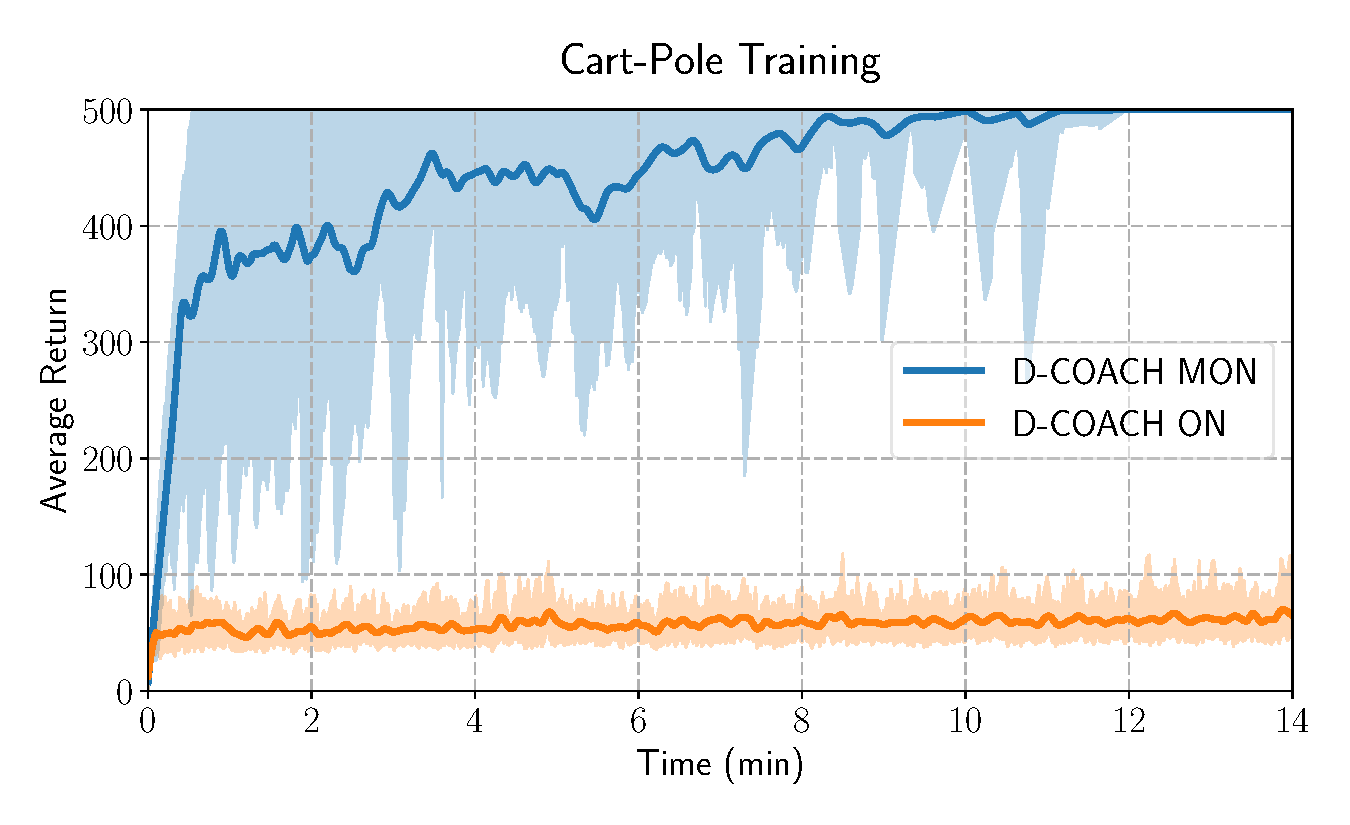
\includegraphics[width=0.7\linewidth]{imagenes/cap3/cartpole_LD_model.pdf}
    \caption[Partially observed Cart-Pole results for simulated teacher comparing D-COACH ON and D-COACH MON.]{Partially observed cart-pole results for simulated teacher comparing D-COACH ON and D-COACH MON.  Buffer: $K = 200$; $k=5$; $b = 10$; $N = 50$; $L=1\mathrm{e}5$; $l=5$; $d=1$; $M=50$; $\tau=8$; $P_{h}$: $\alpha = 0.35$; $\tau = 0.0003$; $\emph{e}=\textbf{1}$. Simulated teacher network learning rate: $0.005$; Transition model learning rate: $0.0005$.}
    \label{fig:ld_cartpole_model}
\end{figure}

D-COACH ON is not able to learn a well performing policy in this case. This was expected, since the velocities of both the cart and the pole are essential for making good decisions in a problem of these characteristics. Figure \ref{fig:cp_ex} shows an example of two scenarios wherein at time step 2 the observation would be the same in the partially observed cart-pole (if we only focus on the angle of the pole). In this example the angular velocity of the pole changes direction between scenarios, but an agent without memory is not able to tell the difference. As a consequence, in $t=2$, it would make the same decision in two opposite scenarios.

\begin{figure}[h]
    \centering
    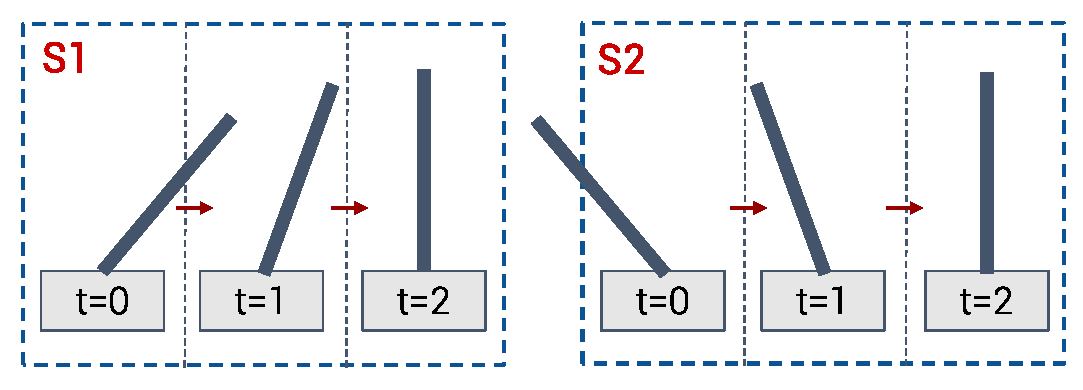
\includegraphics[width=0.7\linewidth]{imagenes/cap4/cartpole_ex.pdf}
    \caption{Cart-pole partial observability example.}
    \label{fig:cp_ex}
\end{figure}

In contrast, if the agent makes decisions based on previous observations it can understand that these two scenarios are different and take better decisions. This is shown in the blue curve of Figure \ref{fig:ld_cartpole_model}, where the agent is able to learn a well performing policy in about 12 minutes. 

\subsection{Validation High-Dimensional State}
In this section, we validate D-COACH MON in two different problems (once again, the simulated teacher training strategy introduced in Chapter 3 is used). Cart-pole is a problem that was not originally designed to be solved using as input raw pixels of an image, so we do not expect to obtain a perfect performance (500 score average). The main goal of testing D-COACH with this problem is to observe if the proposed model (autoencoder + LSTM) is able to embed both the past and high-dimensional inputs adequately.

\begin{figure}[h]
    \centering
    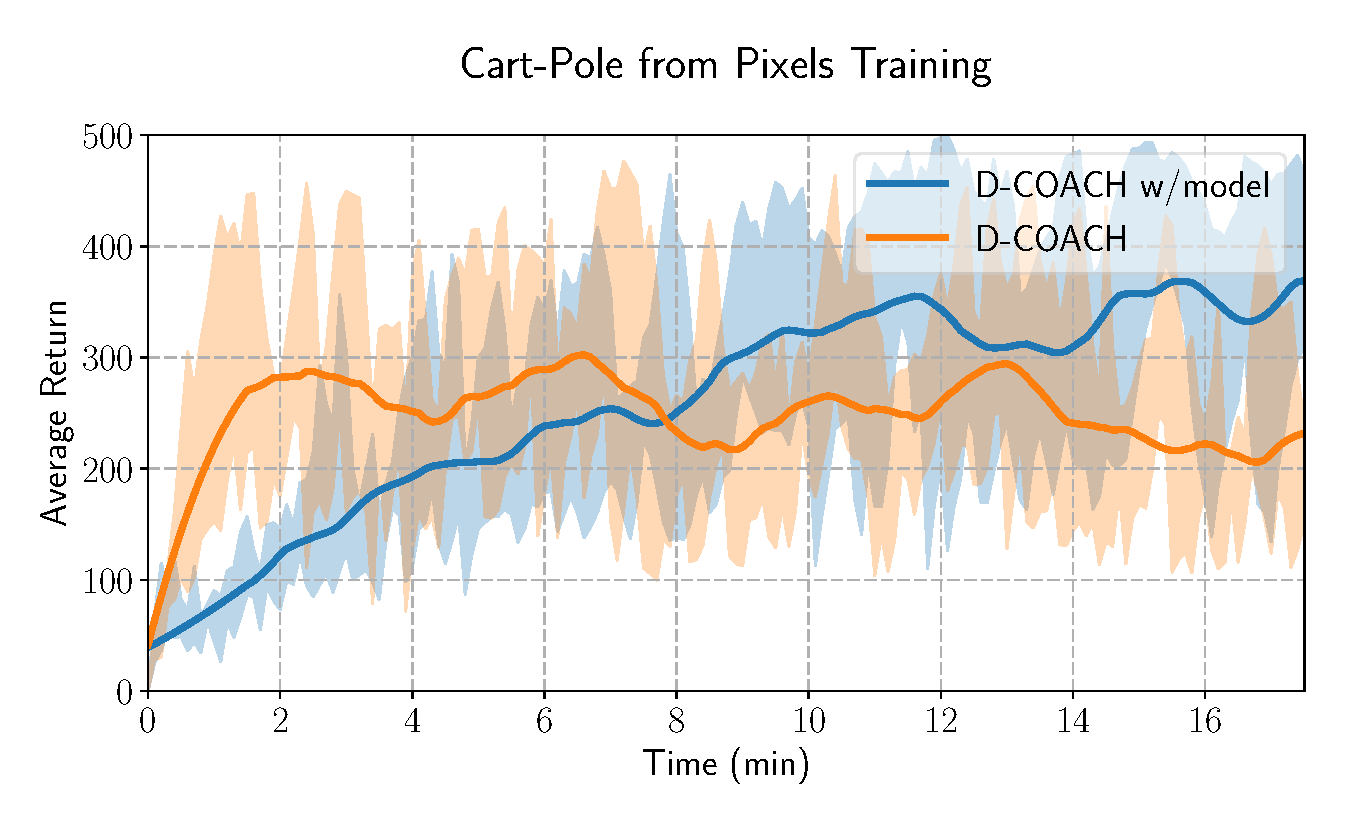
\includegraphics[width=0.7\linewidth]{imagenes/cap3/cartpole_HD_model.pdf}
    \caption[Partially observed Cart-Pole from pixels results for simulated teacher comparing D-COACH ON and D-COACH MON.]{Partially observed cart-pole from pixels results for simulated teacher comparing D-COACH ON and D-COACH MON.  Buffer: $K = 1000$; $k=20$; $b = 1$; $N = 20$; $L=1\mathrm{e}5$; $l=20$; $d=1$; $M=50$; $\tau=4$; $P_{h}$: $\alpha = 0.35$; $\tau = 0.00003$; $\emph{e}=\textbf{1}$; $m=50$; $\epsilon=0.0011$. Simulated teacher network learning rate: $0.0003$; Transition model learning rate: $0.0005$; Autoencoder learning rate: $0.0003$.}
    \label{fig:cp_hd}
\end{figure}

Figure \ref{fig:cp_hd} shows a slower learning speed and a less successful convergence of D-COACH MON if we compare its performance with the one obtained in the low-dimensional observation partially observed Cart-Pole (see Figure \ref{fig:ld_cartpole_model}). This is expected, since in this case the agent must also learn to extract features from the image. Also, D-COACH ON is not able to learn a well performing policy for this problem. So, even though D-COACH MON is not able to achieve the score of 500, a considerable improvement is made over its memoryless version, showing the importance of using recurrency in this type of problems.

Finally, D-COACH MON was validated in the partially observed Car Racing problem. Figure \ref{fig:po_cr} shows that D-COACH ON (orange curve) is able to learn a policy that achieves an average return of $\sim700$ after $\sim15$ minutes of training, which is an acceptable score for this problem. Nevertheless, D-COACH MON (blue curve) shows that it is possible to obtain an even better performance if memory is added to the neural network, achieving an average return of $\sim800$ after $\sim15$ minutes of training (problem is considered to be solved with a score of 900), which is similar to the performance of $\text{D-COACH}$ ON in the fully observable Car Racing (see Figure \ref{fig:simulatedteachers}). The difference between both curves shows that D-COACH MON is a more robust and powerful approach than $\text{D-COACH}$ ON, capable of enhancing the performance of the agent in problems where $\text{D-COACH}$ ON could appear to be sufficient.

\begin{figure}[H]
    \centering
    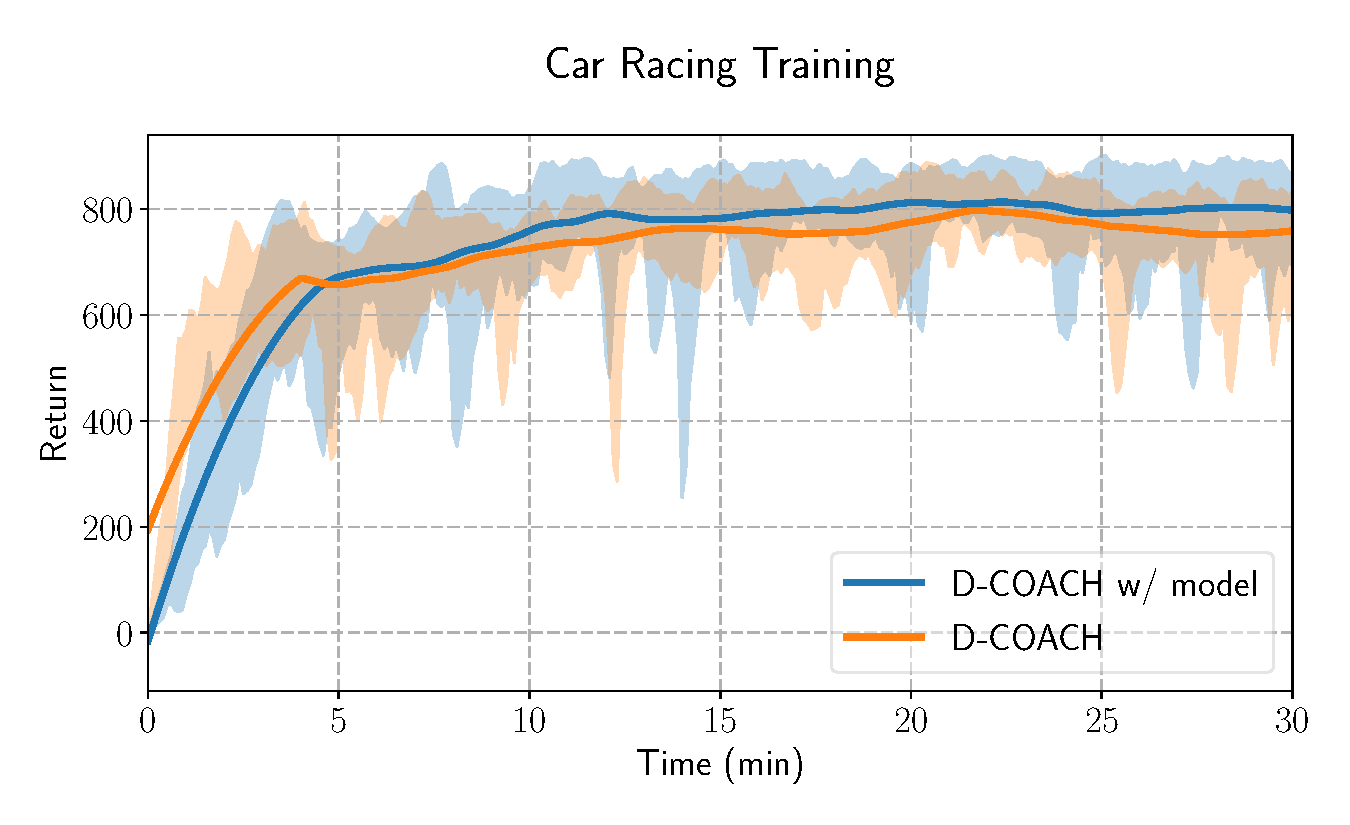
\includegraphics[width=0.7\linewidth]{imagenes/cap3/car_racing_lstm.pdf}
    \caption[Partially observed Car Racing results for simulated teacher comparing D-COACH ON and D-COACH MON.]{Partially observed Car Racing results for simulated teacher comparing D-COACH ON and D-COACH MON.  Buffer: $K = 2000$; $k=20$; $b=10$; $N = 8$; $L=1\mathrm{e}5$; $l=20$; $d=1$; $M=8$; $\tau=10$; $P_{h}$: $\alpha = 0.9$; $\tau = 0.000015$; $\emph{e}=\textbf{1}$; $m=50$; $\epsilon=0.0011$. Simulated teacher network learning rate: $0.003$; Transition model learning rate: $0.0005$; Autoencoder learning rate: $0.003$.}
    \label{fig:po_cr}
\end{figure}

\section{Discussion}
In this chapter we introduced a variation of D-COACH with memory, D-COACH MON. The main objective was to extend D-COACH in order for it to work in the set of POMDPs where the state is described by time-dependent phenomena. Low-dimensional and high-dimensional problems were covered, introducing a different model architecture for each case. 

D-COACH MON offers a framework that learns both the policy and the model online. This makes it easy for humans to interact in the learning process of the agents, given that no human effort is needed in extra learning steps as in the offline state representation learning version of D-COACH (Chapter 3). The experiments show that the proposed method is effective for enhancing the performance of agents in POMDPs. As discussed previously, memory-based approaches may be key to solve problems in real-world scenarios, where is common to face problems with partial observability. 

As it is stated in the overview of this chapter, RNNs have an extra overhead when training, because sequences must be used for updating the weights of the recurrent layers. Given that D-COACH is an IML approach, updates are done in real-time while the teacher is providing feedback. We found that the overhead produced when updating the recurrent layers is too high for running this approach in CPU; thus, a GPU was used. This is a disadvantage with respect to the previously proposed variations of D-COACH, given that those models are able to run in real-time using CPUs. 